\chapter{Sprint 4 – Business Intelligence and Finalization}

\section{Introduction}

In the final sprint, the focus moved from operational functionality to strategic visibility. The goal was to provide administrators with a visual interface to monitor performance, track sales trends, and make data-informed decisions. This was achieved by integrating dashboards built using Microsoft Power BI directly into the application.

Additionally, this sprint included final UI polishing, user experience refinements, and manual system-wide testing to ensure the platform was production-ready.

\section{Sprint 4 Backlog}

\begin{table}[H]
\centering
\begin{tabular}{|c|p{10cm}|c|}
\hline
\textbf{Task ID} & \textbf{Task Description} & \textbf{Status} \\
\hline
S4-T1 & Set up Power BI workspace & Completed \\
S4-T2 & Connect database to Power BI & Completed \\
S4-T3 & Create sales dashboard & Completed \\
S4-T4 & Build product analytics & Completed \\
S4-T5 & Add customer insights & Completed \\
S4-T6 & Create financial reports & Completed \\
S4-T7 & Test dashboard performance & Completed \\
S4-T8 & Deploy BI solution & Completed \\
\hline
\end{tabular}
\caption{Sprint 4 – Backlog and Implementation Plan}
\label{tab:sprint4-backlog}
\end{table}

\section{Business Intelligence Goals}

The integration of BI dashboards aimed to:

\begin{itemize}
  \item Monitor product performance (top sellers, low stock).
  \item Track total revenue and payment breakdowns.
  \item Provide per-cashier activity summaries.
  \item Enable real-time visibility for business stakeholders.
\end{itemize}

Power BI was selected due to its cloud accessibility, ease of integration, and robust data visualization features.

\section{Use Case Diagram}

\begin{figure}[H]
  \centering
  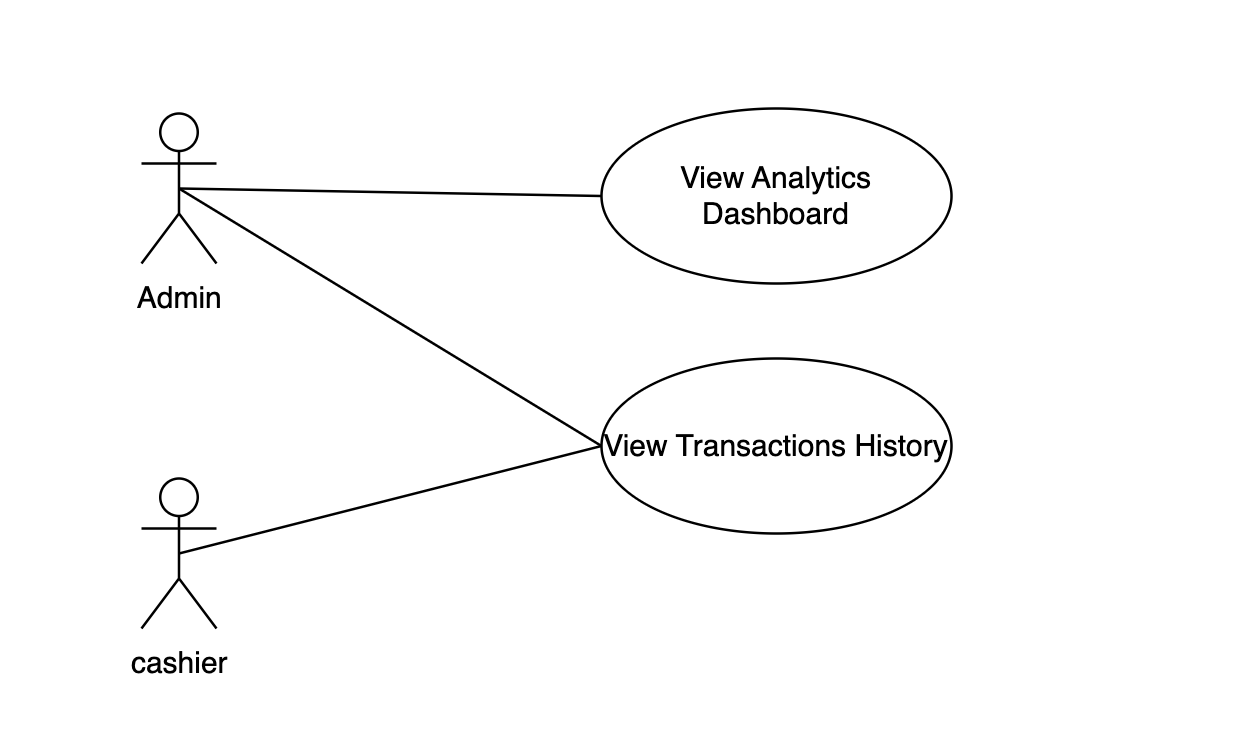
\includegraphics[width=0.9\textwidth]{figures/images/sprint4usecase.png}
  \caption{Sprint 4 – Business Intelligence Use Case Diagram}
  \label{fig:sprint4-usecase}
\end{figure}

\section{Class Diagram}

\begin{figure}[H]
  \centering
  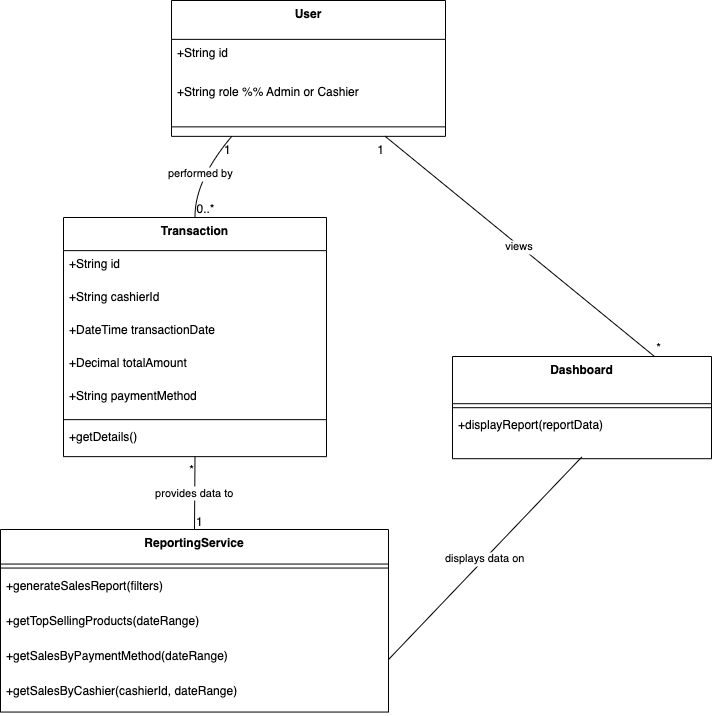
\includegraphics[width=0.9\textwidth]{figures/images/sprint4class.png}
  \caption{Sprint 4 – Business Intelligence Class Diagram}
  \label{fig:sprint4-class}
\end{figure}

\section{Sequence Diagram}

\begin{figure}[H]
  \centering
  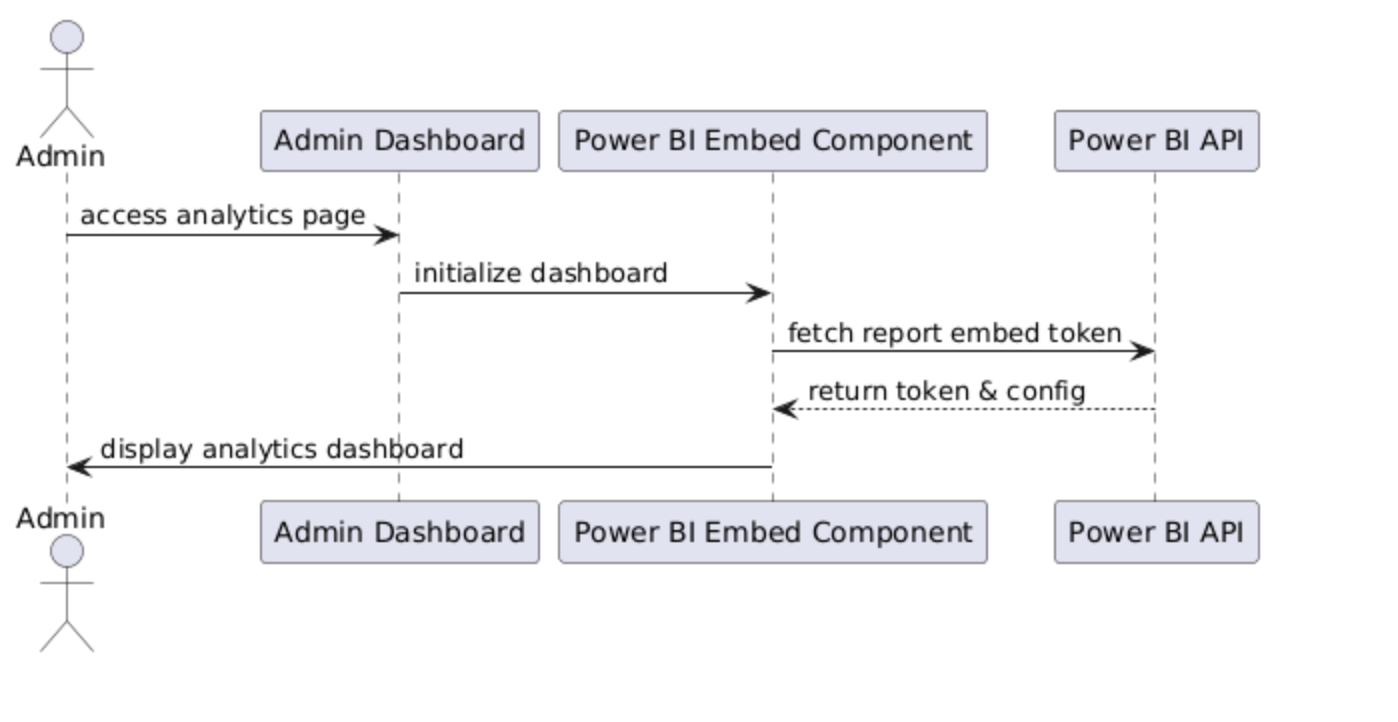
\includegraphics[width=0.9\textwidth]{figures/images/sprint4sequence.png}
  \caption{Sprint 4 – Business Intelligence Integration Sequence Diagram}
  \label{fig:sprint4-sequence}
\end{figure}

The analytics integration sequence demonstrates:
\begin{enumerate}
  \item Admin user accesses the analytics dashboard
  \item System validates admin permissions
  \item Power BI embedded content is loaded
  \item Real-time data is synchronized
  \item Interactive reports are displayed
\end{enumerate}

\section{Implementation Results}

The business intelligence integration was successfully implemented, providing administrators with comprehensive analytics and reporting capabilities.

% Business Intelligence Screenshots
\begin{figure}[H]
  \centering
  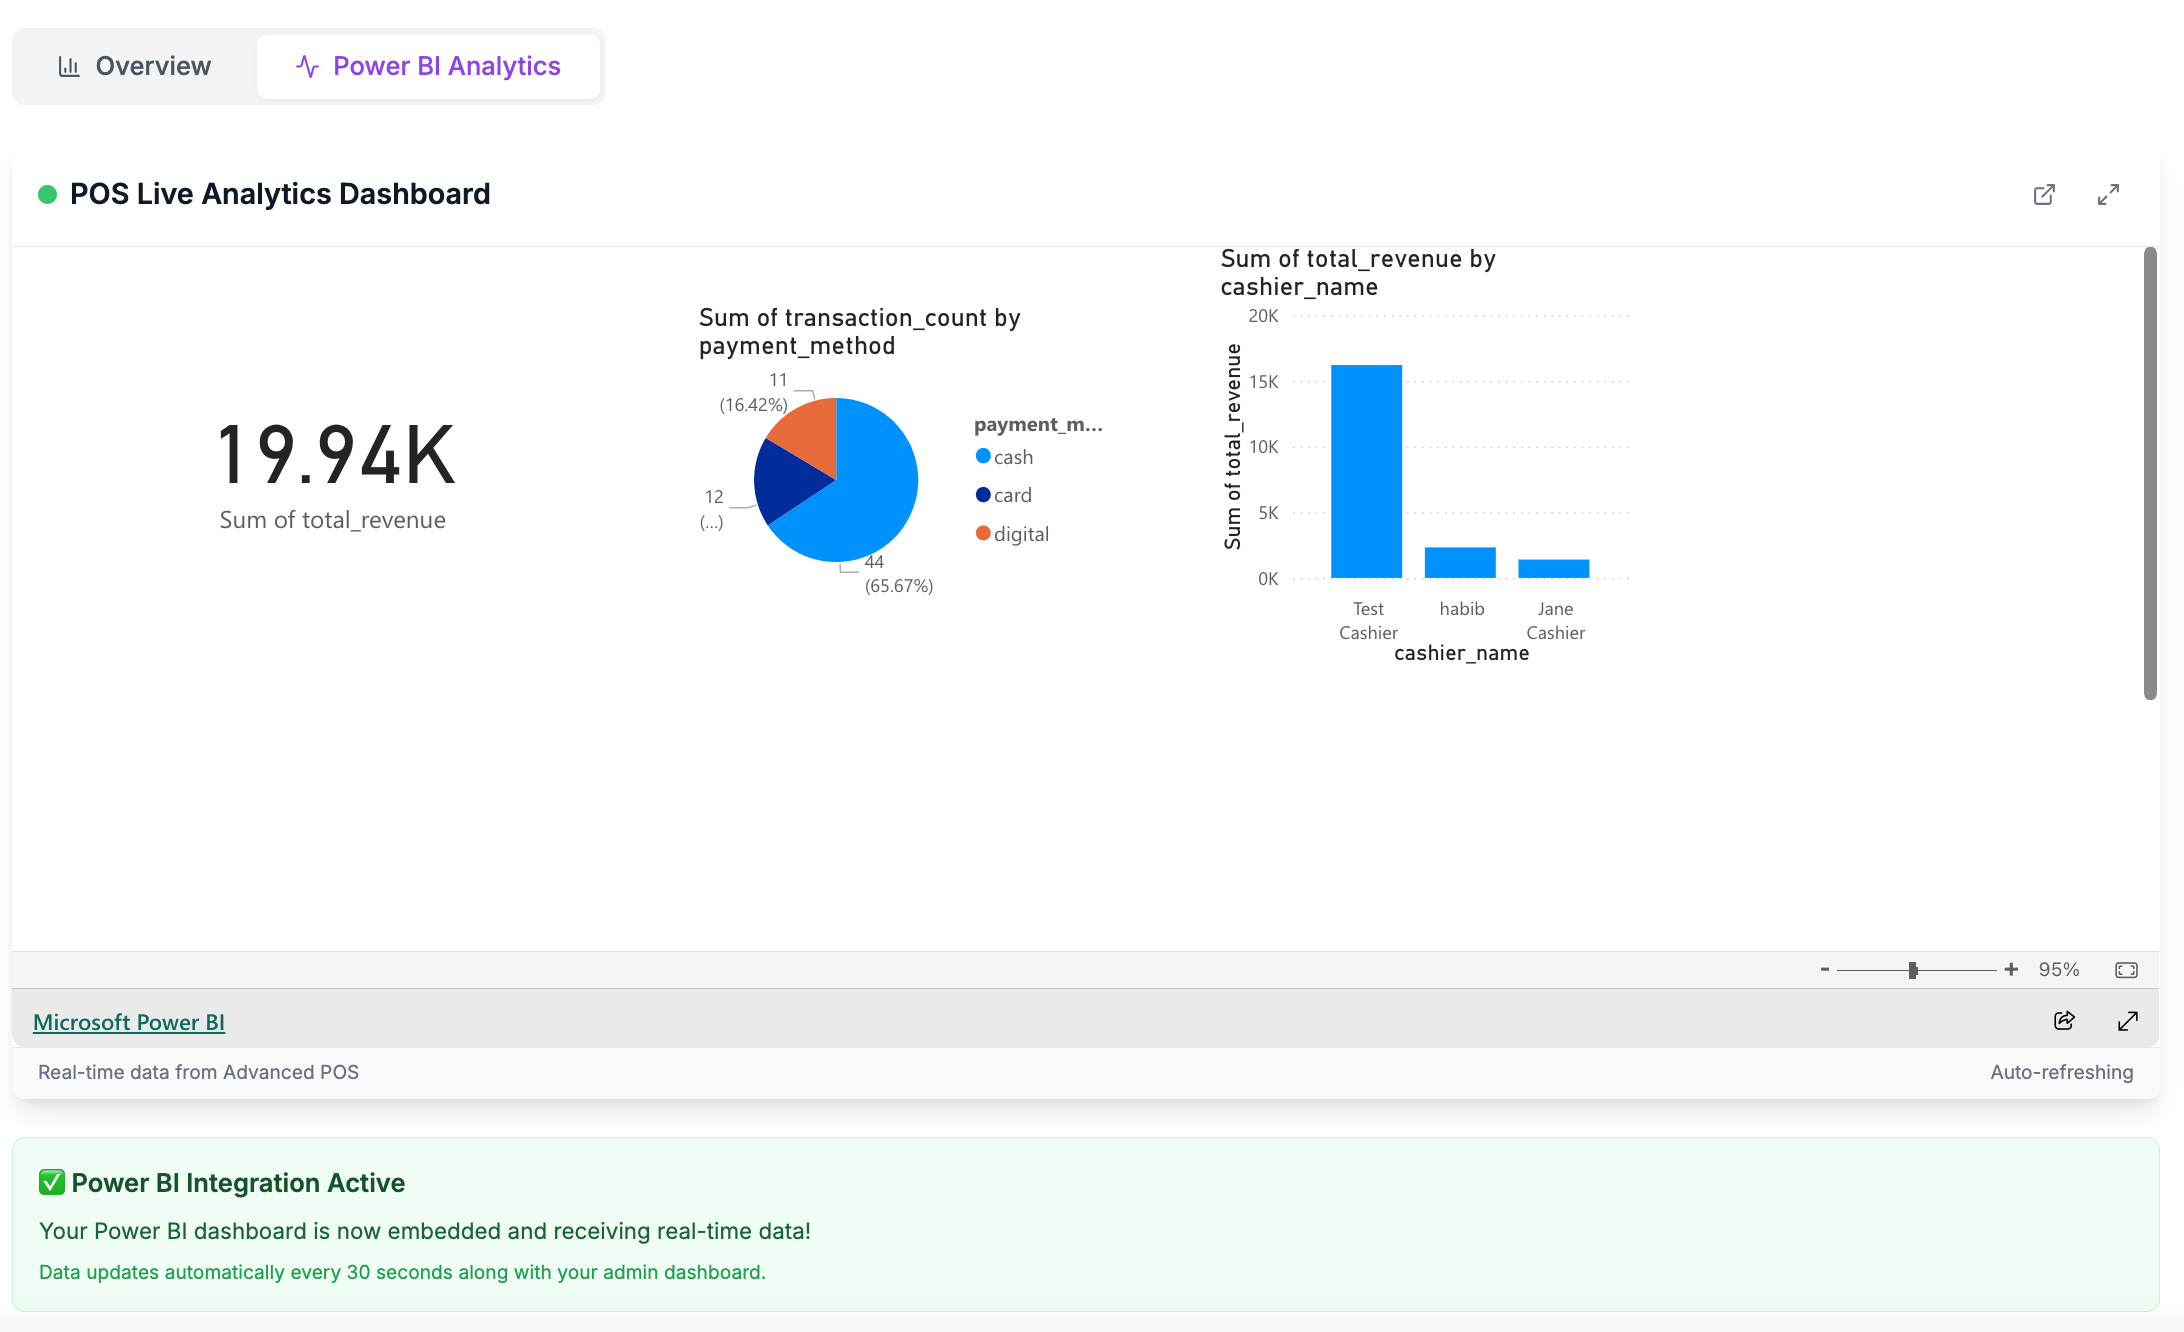
\includegraphics[width=0.9\textwidth]{working app screenshots/powerbiembedded.png}
  \caption{Power BI Dashboard Integration - Embedded analytics with real-time sales and performance metrics}
  \label{fig:powerbiembedded}
\end{figure}

\begin{figure}[H]
  \centering
  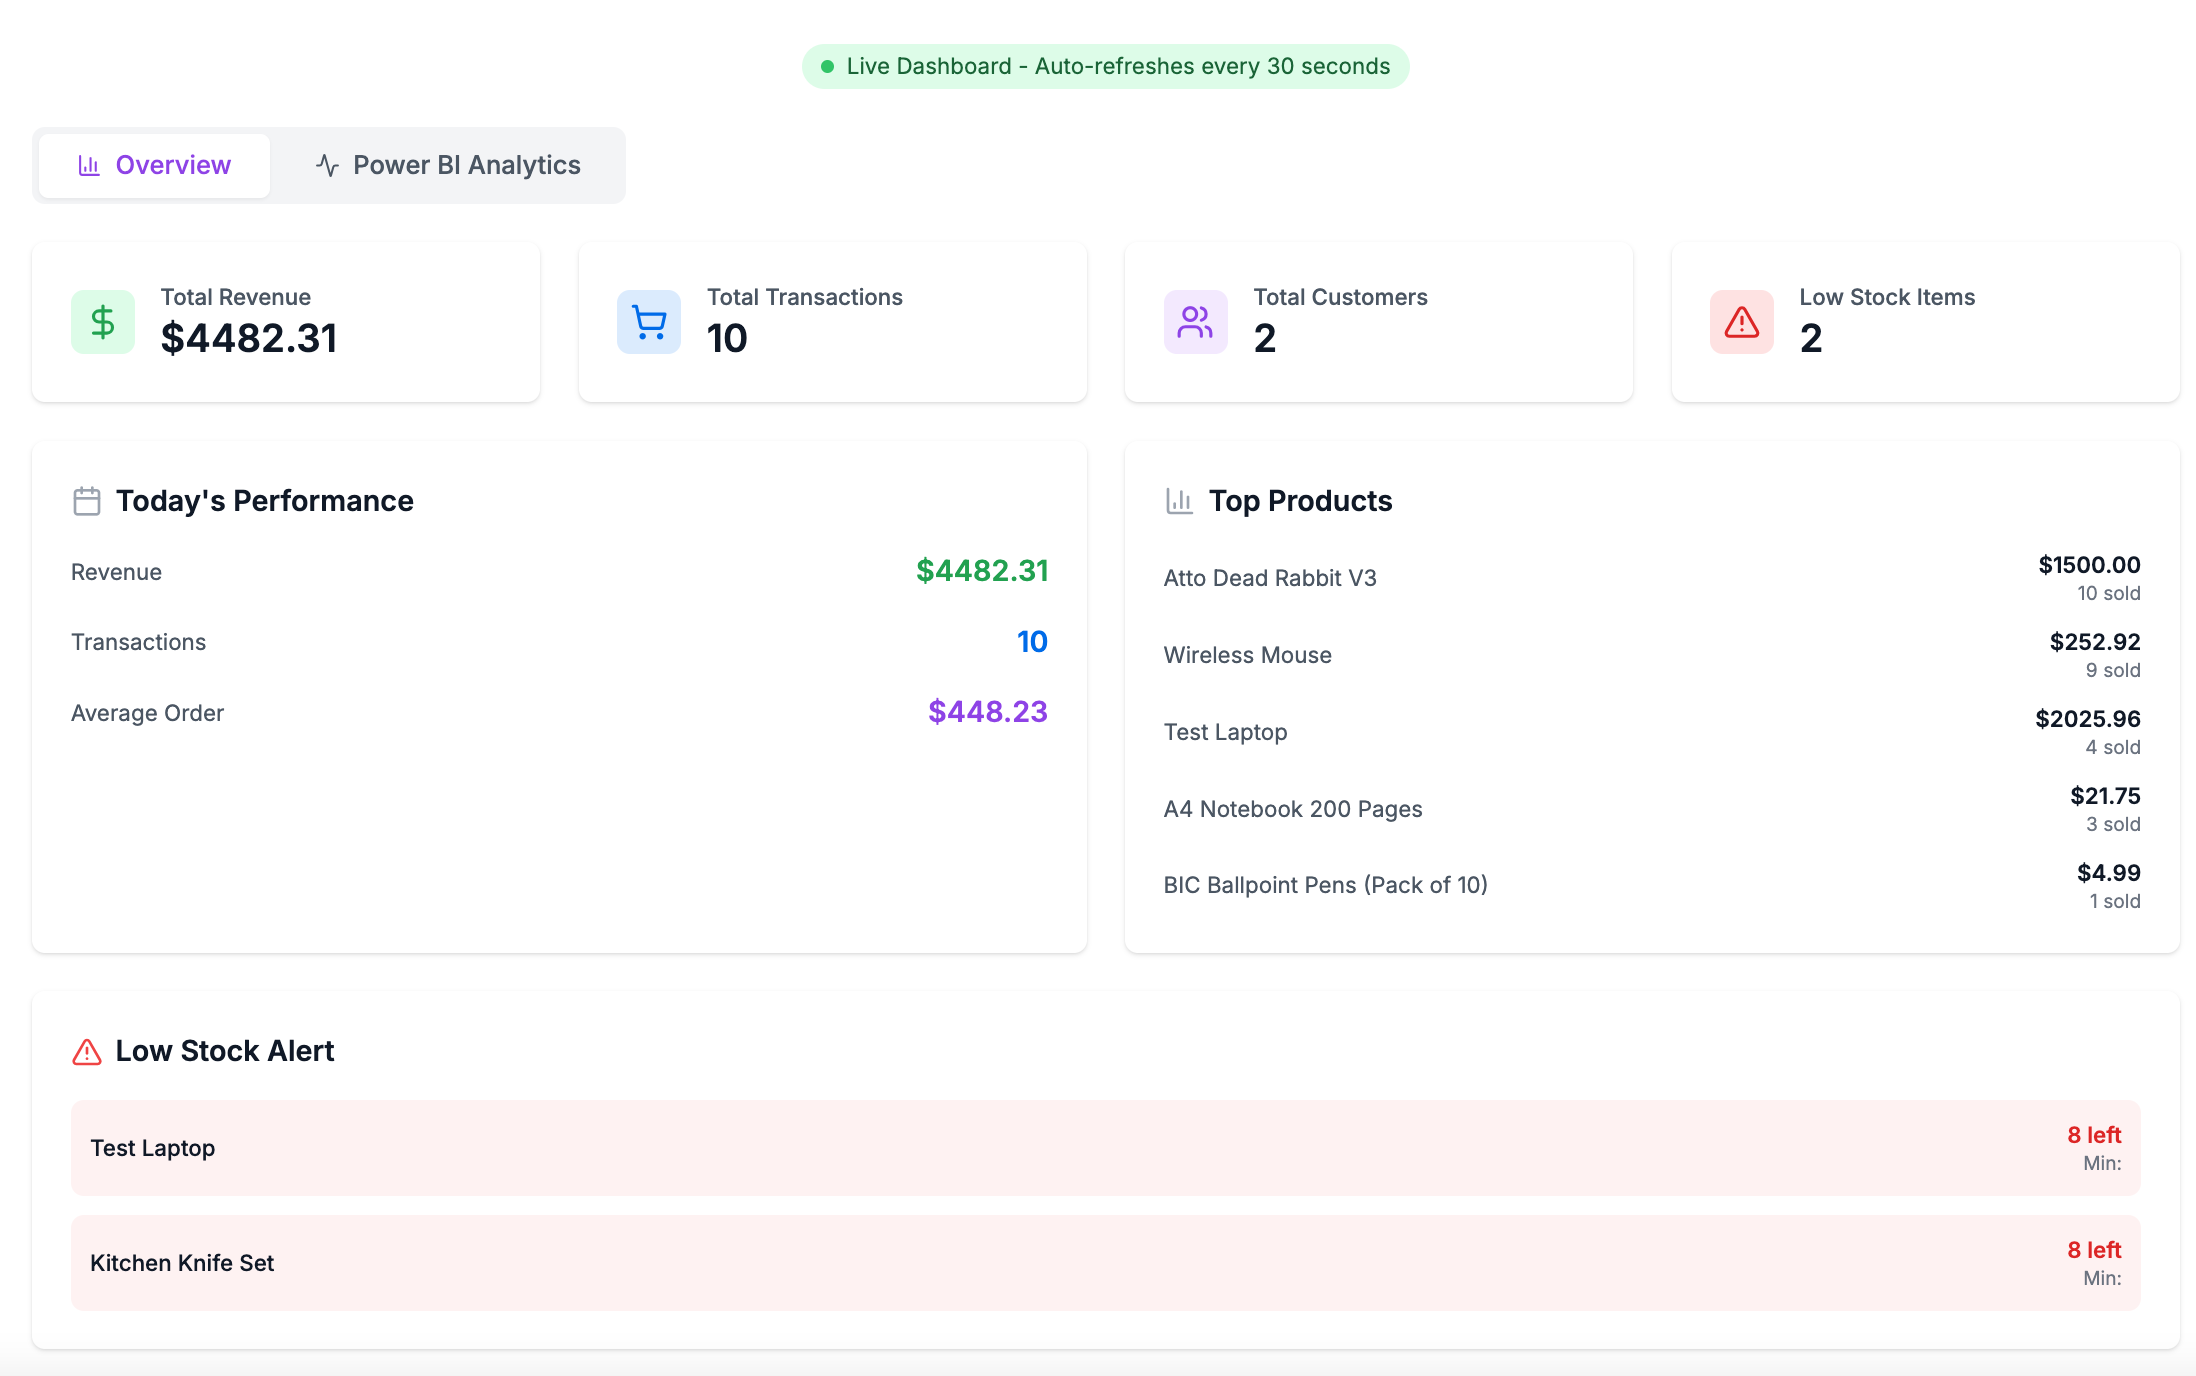
\includegraphics[width=0.9\textwidth]{working app screenshots/salesreports.png}
  \caption{Sales Reports Interface - Comprehensive reporting with charts and filtering options}
  \label{fig:salesreports}
\end{figure}

% Power BI dashboard screenshots removed - to be replaced with new screenshots

The business intelligence integration was successfully implemented with:

\begin{itemize}
  \item Embedded Power BI reports with interactive filtering and real-time data visualization
  \item Comprehensive sales analytics showing revenue trends, top products, and performance metrics
  \item Role-based access control ensuring only authorized administrators can view sensitive business data
  \item Responsive dashboard layout optimized for different screen sizes and devices
  \item Export capabilities for reports and data analysis supporting business decision-making
  \item Real-time data synchronization ensuring analytics reflect current business performance
\end{itemize}

The analytics dashboard provides administrators with comprehensive insights into sales performance, inventory status, and customer behavior patterns, enabling data-driven decision making for business optimization.

% Transaction table screenshot removed - to be replaced with new screenshot

The transaction monitoring interface enables administrators to:
\begin{itemize}
  \item View detailed transaction history
  \item Filter transactions by date, amount, or cashier
  \item Export transaction data for external analysis
  \item Monitor system performance and usage patterns
\end{itemize}

\section{Project Sprint Review}

% Burndown chart removed - to be replaced with new chart

The project followed a structured 4-sprint approach with the following outcomes:

\begin{itemize}
  \item \textbf{Sprint 1:} Authentication and role management - Completed successfully
  \item \textbf{Sprint 2:} User and product management (Admin) - Delivered on schedule
  \item \textbf{Sprint 3:} POS interface and invoicing - Implemented with full functionality
  \item \textbf{Sprint 4:} Business intelligence integration - Completed with Power BI dashboards
\end{itemize}

Each sprint delivered working software increments, allowing for continuous testing and validation throughout the development process.

\section{Conclusion}

Sprint 4 marked the final phase of the POS system development. By embedding Power BI, the application now supports not only operational flows but also decision-making. The platform is fully functional, visually consistent, and aligned with the project objectives.
